
\documentclass[11pt, oneside]{amsart}
\usepackage[utf8]{inputenc}
\usepackage{graphicx}
\usepackage{enumerate}
\usepackage{tikz-cd}
\usepackage{amsmath}
\usepackage{amsthm}
\usepackage{proof}
\usepackage{amssymb,amsmath,amsthm}
\newtheorem{lemma}{Lemma}
\usepackage{amsmath}
\usepackage{multicol}
\usepackage{tikzit}
\usepackage{tikz}
\usepackage{verbatim}
\usepackage{braket}

\newcommand{\ox}{\otimes} 
\newcommand{\oa}{\oplus}

\tikzstyle{strings}=[baseline={([yshift=-.5ex]current bounding box.center)}]
\tikzset{every picture/.append style={scale=.5}, transform shape, strings}
\newtheorem{theorem}{Theorem}
\theoremstyle{definition}
\newtheorem{definition}{Definition}[section]
\theoremstyle{definition}
\newtheorem{exmp}{Example}[section]
\usetikzlibrary{arrows,decorations.pathmorphing,backgrounds,positioning,fit}
\input{rectangular.tikzstyles}
\usetikzlibrary{shapes.arrows}
\tikzset{oa/.style={draw, scale=0.9,minimum height=.1cm,circle,append after command={[shorten >=\pgflinewidth, shorten <=\pgflinewidth,](\tikzlastnode.north) edge(\tikzlastnode.south)(\tikzlastnode.east) edge (\tikzlastnode.west)}}}

 

\tikzset{ox/.style={draw, rotate=45,scale=0.9,minimum height=.1cm,circle,append after command={[shorten >=\pgflinewidth, shorten <=\pgflinewidth,](\tikzlastnode.north) 
edge (\tikzlastnode.south)(\tikzlastnode.east) edge (\tikzlastnode.west)}}}

\tikzstyle{rtriangleb}=[regular polygon, fill=black, regular polygon sides=3, shape border rotate=-90, scale=0.5, draw]
\tikzstyle{ltriangleb}=[regular polygon, fill=black, regular polygon sides=3, shape border rotate=90, scale=0.5, draw]
\tikzstyle{rtrianglew}=[regular polygon,  regular polygon sides=3, shape border rotate=-90, scale=0.5, draw]
\tikzstyle{ltrianglew}=[regular polygon,  regular polygon sides=3, shape border rotate=90, scale=0.5, draw]

\title{The Category CNOT}
\author{Amolak Ratan Kalra }
\date{January 2020}

\begin{document}

\maketitle
\tableofcontents
\section{Introduction}
This report studies the paper The Category CNOT{\cite{robin}}. In this report, I present some properties of restriction categories, inverse categories and discrete inverse categories. These properties are studied as they play a central role in construction of the category CNOT.
\section{Motivation}
The categorical study of the CNOT gate is of central importance in quantum computation because the CNOT gate is responsible for creating entanglement and bell states. A complete set of identities for CNOT helps in quantum circuit optimization and quantum error correction. The categorical perspective is also important in studying the information flow in a quantum circuit. 
\section{CNOT}
The CNOT gate is a two qubit quantum gate. The first bit in a CNOT gate is called the control bit and the second bit is called the target bit. If the control bit is 1 then it flips the target bit otherwise there is no change to either of the bits. The CNOT gate is is one of the fundamental multi qubit gates. The circuit diagram for CNOT is shown in fig 1.
\begin{figure}
    \centering
    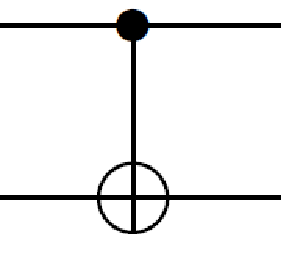
\includegraphics[scale=0.5]{figure8.pdf}
    \caption{Circuit representation of CNOT}
\end{figure}
The matrix of the CNOT gate is given below:
\begin{equation*}
CNOT=
\begin{pmatrix}
1 & 0 & 0 & 0\\
0 & 1 & 0 & 0\\
0 & 0 & 0 & 1\\
0 & 0 & 1 & 0
\end{pmatrix}
\end{equation*}
\section{Categorical Structure of CNOT}
We use ancilla-bits to fix inputs and outputs to be either zero or one. They are
denoted as follows:
\begin{itemize}
    \item Input ancilla and output ancilla for zero
\end{itemize}
\ctikzfig{figure13}
\begin{itemize}
    \item Input and output ancilla for one
\end{itemize}
\ctikzfig{figure14}
\begin{figure}
    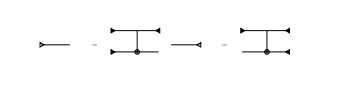
\includegraphics{cnot.PNG}
    \caption{0 state Input and output}
\end{figure}

If we have the one-ancillae and the cnot gate then we do not need the zero-ancilla as:
The ancilla bits and the cnot gate can be used to build circuits by composing the components in parallel or in sequence. This is shown in figure3.
The category CNOT has the following structure.
\begin{itemize}
    \item \textbf{Objects}: Natural Numbers
    \item \textbf{Maps}: Generated by composing ancilla bits and the cnot gates in parallel and in sequence.
\end{itemize}
This forms a symmetric monoidal category. Some identities involving CNOT gates:
\begin{figure}
 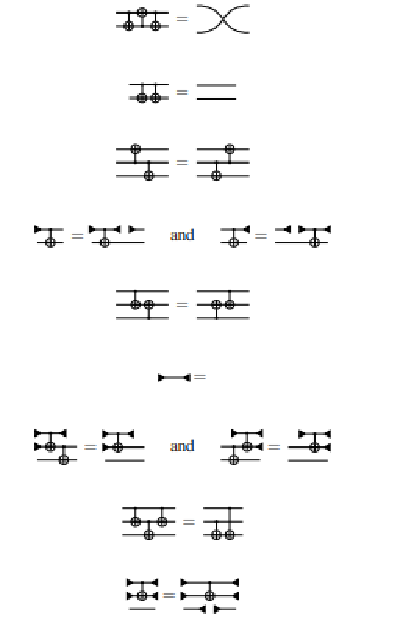
\includegraphics{Identities.pdf}
    \caption{CNOT identities ( This has been taken from the presentation slides)}
\end{figure}
In this report we will understand how we can interpret CNOT as a discrete inverse category.  An inverse category is a type of restriction category so In the next sections we focus on first understanding monoidal categories and subsequently inverse and discrete inverse categories.
\section{Monoidal Categories}
\theoremstyle{definition}
\begin{definition}
A monoidal category $\mathbb{X}$ is a category equipped with:
\begin{itemize}
    \item A bifunctor $\_\otimes{\_}$:$\mathbb{X}\times{\mathbb{X}}\to \mathbb{X}$ is called the \textbf{tensor product}
    \item A distinguished object $I$ of $\mathbb{X}$ called the \textbf{tensor unit}
    \item A natural isomophism a with components $a_{X,Y,Z}:(X\otimes{Y})\otimes{Z} \to X\otimes({Y}\otimes{Z})$ called the \textbf{associator}.
    \item A natural isomorphism $u^{L}$ with components ${u^{L}_{X}}: I\otimes{X}\to X$ called the \textbf{left unitor}
    \item A natural isomorphism $u^{R}$ with components ${u^{R}_{X}}: X\otimes{I}\to X$ called the \textbf{right unitor}.
\end{itemize}
\end{definition}
Such that the following diagrams commute.\\

\textbf{The Maclane Pentagon Diagram}
\begin{equation*}
\centering
\begin{tikzcd}
(({A}\otimes{B})\otimes{C})\otimes{D} \arrow[rr, "{a_{A,B,C}\otimes{1_{D}}}"] \arrow[d, "{a_{A\otimes{B}, C, D}}"] &                                           & (A\otimes{(B\otimes{C}))\otimes{D}} \arrow[rr, "{a_{A,{B\otimes{C},D}}}"] &  & {A}\otimes((B\otimes{C}\otimes{D}) \arrow[d, "{a_{1\otimes{a}_{B, C, D}}}"] \\
(A\otimes{B})\otimes(C\otimes{D}))                                                                                 & {} \arrow[rrr, "{a_{A, B, C\otimes{D}}}"] &                                                                           &  & A\otimes{(B\otimes(C\otimes{D}))}                                          
\end{tikzcd}
\end{equation*}
\textbf{Interaction of unitors and associator:}
\begin{equation*}
\begin{tikzcd}
({A}\otimes{I})\otimes{B} \arrow[rr, "{a_{A,I,B}}"] \arrow[rd, "{u^{R}_{A}}\otimes{1_{B}}"] &               & {A}\otimes({I}\otimes{B}) \arrow[ld, "1_{A}\otimes{{u^{L}_B}}"] \\
                                                                                            & (A\otimes{B}) &                                                                
\end{tikzcd} 
\end{equation*}

A monoidal category is said to be \textbf{symmetric} if additionally it is equipped with a natural isomorphism c with components $c_{X,Y}: {X}\otimes{Y} \to {Y}\otimes{X}$ called the \textbf{symmetry} such that
the following diagrams commute:\\

\textbf{Inverse Law}:
\begin{equation*}
\begin{tikzcd}
{A}\otimes{B} \arrow[d, "{c_{A,B}}"] \arrow[rd, Rightarrow] &             \\
B\otimes{A} \arrow[r, "{C_{B,A}}"]                          & A\otimes{B}
\end{tikzcd}
\end{equation*}
\textbf{Interaction of symmetry with unitors}
\begin{equation*}
\begin{tikzcd}
A\otimes{I} \arrow[r, "{c_{A,I}}"] \arrow[d, "{u^{R}_A}"] & I\otimes{A} \arrow[ld, "{u^{L}_{A}}"] \\
A                                                         &                                      
\end{tikzcd}
\end{equation*}
\textbf{Interaction of symmetry with associator}
\begin{equation*}
\begin{tikzcd}
(A\otimes{B})\otimes{C} \arrow[d, "{a_{A,B,C}}"] \arrow[rr, "{c_{A,B}\otimes{1_{C}}}"] &  & ({B}\otimes{A)}\otimes{C} \arrow[d, "{a_{B,A,C}}"]             \\
A\otimes({B}\otimes{C}) \arrow[d, "{c_{A,{B\otimes{C}}}}"]                             &  & {B}\otimes({A}\otimes{C}) \arrow[d, "{1_{B}\otimes{c_{A,C}}}"] \\
(C\otimes{B})\otimes{A} \arrow[rr, "{a_{A,B,C}}"]                                      &  & {B}\otimes({C}\otimes{A})                                     
\end{tikzcd}
\end{equation*}
%\section{Restriction Categories}
%A restriction structure on a category \textit{X} is an assignment $\overline{f}: A \to A$ for each map $f: A \to B$ in \textit{X} satisfying the four axioms:
%\begin{itemize}
    %\item $\overline{f}{f}=f$ for every map f in \textit{X} 
    %\item $\overline{f}\overline{g}=\overline{g}\overline{f}$ whenever dom($f$)=dom($g$) for maps $f$ and $g$ in \textit{X}
    %\item $\overline{\overline{g}{f}}=\overline{f}\overline{g}$ whenever dom($f$)=dom($g$) for maps $f$ and $g$ in \textit{X}
    %\item ${f}\overline{g}=\overline{fg}f$ whenever dom($f$)=dom($g$) for maps $f$ and $g$ in \textit{X}\end{itemize}
\section{Restriction Categories}
We now study some properties of restriction categories. The description closely follows that given in \cite{brett}.\\
\begin{definition}
 A \textbf{restriction category} is a category $\mathbb{X}$  together with a  restriction operator on maps,\\
\begin{equation*}
\infer{\overline{f}: A \to A} {f: A \to B} 
\end{equation*}
 where f is a map of $\mathbb{X}$ and A, B are objects of $\mathbb{X}$ such that the following four restriction identities hold whenever composition is defined:
\begin{equation*}
\overline{f}{f}=f \tag{R1}
\end{equation*}
\begin{equation*}
\overline{f}\overline{g}=\overline{g}\overline{f} \tag{R2}
\end{equation*}
\begin{equation*}
\overline{\overline{g}{f}}=\overline{f}\overline{g} \tag{R3}
\end{equation*}
\begin{equation*}
{f}\overline{g}=\overline{fg}f \tag{R4}
\end{equation*}
\end{definition}
\begin{definition}
 A \textbf{restriction functor} is a functor which preserves the restriction. That is given a functor $F$: $\mathbb{X} \to \mathbb{Y}$ with $\mathbb{X}$ and $\mathbb{Y}$ restriction categories, $F$ is a restriction functor if:\\
\begin{equation}
F(\overline{f})=\overline{F(f)}
\end{equation}
Note that any map such that $r=\overline{r}$ is an idempotent as $rr=\overline{r}r=r$. Such a map is called a \textbf{restriction idempotent}.
\end{definition}
\begin{lemma}
In a restriction category $\mathbb{X}$

\begin{multicols}{2}
\begin{enumerate}[(i)]
\item $\overline{f}$ is idempotent;            
\item $\overline{fg}={\overline{fg}}$ $\overline{f}$;
\item $\overline{fg}=\overline{f\overline{g}}$;
\item $\overline{\overline{f}}=\overline{f}$;
\columnbreak

\item $\overline{f}\overline{g}=\overline{\overline{f}\overline{g}}$;
\item f monic implies $\overline{f}=1$;
\item ${f=\overline{g}f \implies \overline{g}\overline{f}=\overline{f}}$

\end{enumerate}
\end{multicols}


%\item $\overline{f}$ is idempotent;            
%\item $\overline{fg}={\overline{fg}}$ $\overline{f}$;
%\item $\overline{fg}=\overline{f\overline{g}}$;
%\item $\overline{\overline{f}}=\overline{f}$;
%\item $\overline{f}\overline{g}=\overline{\overline{f}\overline{g}}$;
%\item f monic implies $\overline{f}=1$;
%\item ${f=\overline{g}f \implies \overline{g}\overline{f}=\overline{f}}$

\end{lemma}
\begin{proof}~
\begin{enumerate}[(i)]
\item We need to show that $\overline{f}$ is idempotent, this is equivalent to showing that $\overline{f}\overline{f}=\overline{f}.$\\
$\overline{f}\overline{f}\stackrel{\text{(R3)}}{=}\overline{\overline{f}f}\stackrel{\text{(R1)}}{=}\overline{f}$.
\item We have $\overline{fg}\stackrel{\text{(R1)}}{=}\overline{{\overline{f}fg}}\stackrel{\text{(R3)}}{=}\overline{f}\overline{fg}\stackrel{\text{(R2)}}{=}\overline{fg}$ $\overline{f}$
\item $\overline{fg}\stackrel{\text{Lemma 1(ii)}}{=}$ $\overline{fg}$ $\overline{f}$ $\stackrel{\text{(R3)}}{=}\overline{\overline{fg}f}\stackrel{\text{(R4)}}{=}\overline{f\overline{g}}$
\item $\overline{f}=\overline{1f}\stackrel{\text{(lemma 1 (iii))}}{=}{\overline{1\overline{f}}=\overline{\overline{f}}}$\\
The first and last equality follow from the fact that $\mathbb{X}$ is a category and satisfies the unit law of a category.
\item $\overline{\overline{f}\overline{g}}\stackrel{\text{(R3)}}{=}\overline{f}\overline{{\overline{g}}}\stackrel{\text{(lemma 1) (iv)}}{=}\overline{f}\overline{g}$
\item $\overline{f}{f}\stackrel{\text{(R1)}}{=}f=1f$ now we are given that f is monic this implies $\overline{f}=1$
\item $\overline{g}\overline{f}\stackrel{\text{(R3)}}{=}\overline{\overline{g}f}$. We already assume that $f=\overline{g}f$ this implies that $\overline{\overline{g}f}=\overline{f}$
\end{enumerate}
\end{proof}

\begin{exmp}
(PAR): This is the subcategory of Rel which has the same objects (sets)
but only allowing maps which are partial functions, i.e., deterministic relations $f$ where if $(x,y), (x,y^{\prime}) \in f$ then $y=y^{\prime}$.PAR is a restriction category. The restriction of $f: A \to B$ is:
\begin{equation*}
    \overline{f(x)}=
    \begin{cases}
    x & \text{if $f(x)$ is defined}\\
    \uparrow & \text{if $f(x)$ is undefined}
    \end{cases}
\end{equation*}
In PAR the total maps correspond precisely to the functions that are defined on all elements of the domain.\\
\end{exmp}
\begin{exmp}
(REL): The category REL is the following:
\begin{itemize}
    \item \textbf{Objects}: All Sets
    \item \textbf{Maps}: $R: X \to Y$ is a relation : $R \subseteq X\times{Y}$
    \item \textbf{Identity}: $1_{X}=\{(x,x)|x \in X\}$
    \item \textbf{Composition}: $RS=\{(x,z)|\forall{y}, (x,y)\in R$ and $(y,z) \in  S\}$
\end{itemize}
The category REL is not a restriction category with candidate restriction of $R={(a,b)}$ being $\overline{R}={(a, a)|\exists b (a,b)\in R}$. The axiom that fails is (4).\\
\end{exmp}
\begin{exmp}
(PINJ):The category PINJ consists of the partial injective functions over sets. Similarly
to Sets and Par, it is a subcategory of REL. The maps f, g (relations in REL) in PINJ are
subject to two condition:
\begin{itemize}
    \item $(x,y) \in f$ and $(x,y^{\prime}) \in f$ implies $y=y^{\prime}$
    \item $(x,y) \in f$ and $(x^{\prime},y) \in f$ implies $x=x^{\prime}$
\end{itemize}
We see that PINJ is a restriction category it is in fact a subrestriction category of PAR.
\begin{itemize}
    \item $\{\overline{f}f={{(x,z)|\exists x. (x,x) \in f}\}=\{{(x,z)|(x,z) \in f}\}=f}$
    \item ${\overline{f}\overline{g}=\{(x,z)|\exists y.(x,y)\in \overline{f} \text{and} (y,z) \in \overline{g}\}=\{(x,x)|(x,x) \in \overline{f} \text{and} (x,x) \in \overline{g}\}=\overline{g}\overline{f}}$
    \item ${\overline{\overline{f}g}=\overline{\{(x,y)|(x,x) \in \overline{f}, (x,y)\in g\}}}$=$\overline{f}\overline{g}$
    \item $f\overline{g}=\{(x,y)|(x,y) \in f, (y,y) \in \overline{g}\}=\{(x,y)|(x,y)\in f,\exists z.(y,z)\in g\}=\{(x,y)|(x,y)\in f,\exists z.(x,z)\in fg\}=\{(x,y)|(x,y)\in f,(x,x)\in \overline{fg}\}$
    \end{itemize}
    % Axiom 4 needs to be shown
\end{exmp}

\section{Cartesian Restriction Category}
\begin{definition}
 In a \textbf{restriction category} $\mathbb{X}$ a restriction product of two objects $X$ and $Y$ is an object $X\times Y$ equipped with total projections $\pi_{0}: X \times Y \to X$, $\pi_{1}:X \times Y \to Y $ where\\
\begin{equation*}
\forall f: Z \to X, g: Z \to Y \exists \text{a unique} \langle{f,g}\rangle : Z: X \to X \times Y 
\end{equation*}
such that
\begin{itemize}
    \item $\langle{f,g}\rangle\pi_{0}\leq f$
    \item $\langle{f,g}\rangle\pi_{1}\leq g$
    \item $\overline{\langle{f,g}\rangle}=\overline{f}\overline{g}$
\end{itemize}
\end{definition}
\begin{definition}
 In a restriction category $\mathbb{X}$ a \textbf{restriction terminal object} is an object $T$ such that for all objects $X$ there is a unique map $!_{X}: X \to T$ and the diagram below commutes:\\
\begin{equation*}
\begin{tikzcd}
X \arrow[r, "\overline{f}"] \arrow[d, "f"] & X \arrow[r, "!_{X}"] & T \\
Y \arrow[rru, "!_{Y}"]                     &                      &  
\end{tikzcd}
\end{equation*}
That is $f!_{Y}=\overline{f}!_{X}$\\
\end{definition}


\begin{definition}
 A restriction category $\mathbb{X}$ is \textbf{Cartesian} if it has all restriction products and a restriction terminal object
\end{definition}
\begin{definition}
 An object $A$ in a Cartesian restriction category is \textbf{discrete} when the diagonal map 
\end{definition}
\begin{equation*}
\Delta: A \to A \times A
\end{equation*}
is a partial isomorphism. A Cartesian restriction category where all objects are discrete is called a discrete  Cartesian restriction category \\
\textbf{Example}(PAR is discrete): In PAR
\begin{equation*}
    \Delta: x \mapsto (x,x) \ \text{and}\ \Delta^{-1}: (x,y) \mapsto 
    \begin{cases}
    x & \text{$x=y$}\\
    \uparrow & \text{x $\neq$ y}
    \end{cases}
\end{equation*}
Thus PAR is a discrete Cartesian restriction category.\\
\begin{exmp}
Terminal object is discrete: In any Cartesian restriction category the terminal object 1 is discrete because $1 \times 1 \cong 1$
\end{exmp}
\section{Inverse Categories}
\begin{definition}
 In a restriction category $\mathbb{X}$ a map $f$ is said to be a \textbf{partial isomorphism} when there is a partial inverse written $f^{(-1)}$ with $ff^{(-1)}=\overline{f}$ and $f^{(-1)}f=\overline{f^{(-1)}}$
\end{definition}
\begin{definition}
 A \textbf{restriction category} in which every map is a partial isomorphism is
called an \textbf{inverse category}.
\end{definition}
\begin{lemma}
In an inverse category all idempotents are restriction idempotents
\begin{proof}
Given an idempotent $e$;\\
$\overline{e}=e{e^{(-1)}}=ee{e^{(-1)}}=e\overline{e}=\overline{ee}e=\overline{e}e=e$
\end{proof}
\end{lemma}
\begin{exmp}
(PINJ is an inverse category):  For any map $f$, $f^{-1}= {\{(y,x)|(x,y)\in f\}}$
Note that $f^{-1}$ is a map in PINJ.\\
\end{exmp}
\begin{exmp}
(PAR is not an inverse category): PAR while it is an inverse category it is not a restriction category. For example let $X=\{(1,2)\}$ and $Y=\{1\}$ and $f=\{(1,1), (2,1)\}$ in PAR
The restriction of $f$ is $\overline{f}=\{(1,1),(2,2)\}=1_{A}$. There is no partial function $g:B \to A$ such that $fg=1_{A}$\\
\end{exmp}
\begin{exmp}
Generally  let $\mathbb{R}$ be a restriction category and {INVR} the subcategory of $\mathbb{R}$ having the same objects as $\mathbb{R}$ but only partial isomorphisms as maps. Then {INVR} is an inverse category\\
\end{exmp}
\begin{exmp}
A groupoid, which is a category in which every map is an isomorphism, is
an inverse category. As all maps in the groupoid are total, the partial isomorphisms are all
isomorphisms.
\end{exmp}
Alternatively we have the following theorem:
\begin{theorem}
For a category $\mathbb{X}$ the following are equivalent:
\begin{enumerate}[(i)]
    \item $\mathbb{X}$ is an inverse category that is, it has restriction structure for which every map is a restricted isomorphism.
    \item Every morphism $f:A \to B$ has a unique $g:B \to A$ with $fgf=f$ and $gfg=g$
    \item There is a functor $(\_)^{op}: \mathbb{X} \to {\mathbb{X}^{op}}$ which is the identity on objects and satisfies:
    \begin{itemize}
        \item $(f^{o})^{o}=f$
        \item $ff^{o}f=f$
        \item $ff^{o}gg^{o}=gg^{o}ff^{o}$
    \end{itemize}
\end{enumerate}
Here $f^{o}$ denotes the restricted inverse. 
\begin{proof}~
\begin{enumerate}[(i)]
    \item $(i) \implies (ii)$ Suppose in an inverse category we have $fgf=f$ and $gfg=g$
 we must establish that g is the restricted inverse $f^{o}$ of f.\\
 First note that $\overline{g}f=f\overline{gf}=fgf\overline{gf}=fgf=f$ and so $\overline{gf}=\overline{\overline{g}f}=\overline{f}$. For any idempotent $e$ we have $e=e\overline{e}=e\overline{ee}=\overline{e}e=e^{o}ee=e^{o}e=\overline{e}$ and so all idempotents are restriction idempotents. Thus $gf=\overline{gf}=\overline{f}$ and similarly $fg=\overline{g}$.
 Now using the fact that restriction idempotents commute we have $g=gfg=gff^{o}fg=gfgff^{o}=gff^{o}ff^{o}=f^{o}ff^{o}=f^{o}$
 \item $(ii) \implies (iii)$ Define $f^{o}$ to be a unique arrow satisfying $ff^{o}f=f$ and $f^{o}ff^{o}$. We need to show that $ff^{o}gg^{o}=gg^{o}ff^{o}$ and functoriality.
 We shall prove that all idempotents commute from which it follows that $ff^{o}gg^{o}=gg^{o}ff^{o}$. Let e and $e^{\prime}$ be idempotents and let $x=(e^{\prime}e)^{o}$ and then $e^{\prime}exe^{\prime}e=e^{\prime}e$ and $xe^{\prime}ex=x$. Now $(exe^{\prime})^{2}=exe^{\prime}$ and so $exe^{\prime}$ is an idempotent giving $(exe^{\prime})^{o}=exe^{\prime}$. Also $(e^{\prime}e)(exe^{\prime})(e^{\prime}e)=e^{\prime}e$, 
 $(exe^{\prime})(e^{\prime}e)(exe^{\prime})=(exe^{\prime})$ and so $e^{\prime}e=(exe^{\prime})^{o}$ and so $(e^{\prime}e)^{o}=e^{\prime}e$. We then have $(e^{\prime}e)(ee^{\prime})(e^{\prime}e=ee^{\prime}$. Similarly we have $(ee^{\prime})(e^{\prime}e)(ee^{\prime})=ee^{\prime}$. From this we have $e^{\prime}e=(e^{\prime}e)^{o}=ee^{\prime}$\\
 For functoriality we have $gff^{o}g^{o}gf=gg^{o}gff^{o}f=gf$ and $f^{o}ff^{o}g^{o}gg^{o}=f^{o}g^{o}$ and similarly $1^{o}=1$
 \item $(iii) \implies (i)$ We set $\overline{x}=x^{o}x$ then (R1) and (R2) follow. Under this definition each arrow is a restricted isomorphism. For (R3) we have \\
 $\overline{g\overline{f}}=(gf^{o}f)^{o}gf^{o}f=f^{o}fg^{o}gf^{o}f=g^{o}gf^{o}f=\overline{g}\overline{f}$
 Finally for (R.4) we have 
 $\overline{g}f=g^{o}gf=g^{o}gff^{o}f=ff^{o}g^{o}gf=f(gf)^{o}=f\overline{gf}$
 \end{enumerate}

\end{proof}
\end{theorem}
\textbf{Definition}: Given an \textbf{inverse category} $\mathbb{X}$ equipped with a tensor product ${-}\otimes{-}: \mathbb{X} \times \mathbb{X} \to \mathbb{X}$ which preserves $(-)^{o}$ we say X has inverse products if there exists a total diagonal natural transformation $\Delta$ which satisfies the following properties:

Cocommutativity:
\begin{equation*}
\begin{tikzcd}
A \arrow[rrr, "\Delta_{A}"] \arrow[rrrdd, "\Delta_{A}"] &  &  & A\otimes{A} \arrow[dd, "{c_{A, A}}"] \\
                                                        &  &  &                                     \\
                                                        &  &  & D                                  
\end{tikzcd}
\end{equation*}
Coassociativity:
\begin{equation*}
\begin{tikzcd}
A \arrow[rrrrr, "\Delta_{A}"] \arrow[dd, "\Delta_A"] &  &  &                         &  & A\otimes{A} \arrow[dd, "1_{A}\otimes{\Delta_{A}}"] \\
                                                     &  &  &                         &  &                                                    \\
A\otimes{A} \arrow[rrrd, "{\Delta_A}\otimes{1_A}"]   &  &  &                         &  & A\otimes(A\otimes{A)} \arrow[lld, "{a_{A, A, A}}"] \\
                                                     &  &  & (A\otimes{A})\otimes{A} &  &                                                   
\end{tikzcd}
\end{equation*}
Frobenius Algebra:
\begin{equation*}
\begin{tikzcd}
A\otimes{A} \arrow[rrr, "{(\Delta_{A}\otimes{1_{A}})a_{A,A,A}}"] \arrow[dd, "{(1_{A}\otimes{\Delta_{A}}){a^o}_{A,A,A}}"] \arrow[rrd, "{\Delta_{A}}"] &  &                            & {A}\otimes({A}\otimes{A}) \arrow[dd, "1_{A}\otimes{\Delta{^o}_{A}}"] \\
                                                                                                                                                     &  & A \arrow[rd, "\Delta_{A}"] &                                                                      \\
({A}\otimes{A})\otimes{A} \arrow[rrr, "{\Delta{^o}_{A}}\otimes1_{A}"]                                                                                &  &                            & {A}\otimes{A}                                                       
\end{tikzcd}
\end{equation*}
\begin{equation*}
\begin{tikzcd}
{A}\otimes{B} \arrow[rrr, "\Delta_{A}\otimes{\Delta_{B}}"] \arrow[rrdd, "\Delta_{A\otimes{B}}"] &  &                                       & (A\otimes{A})\otimes(B\times{B}) \arrow[ldd, "{ex_{A,B}}"] \\
                                                                                                &  &                                       &                                                            \\
                                                                                                &  & ({A}\otimes{B})\otimes({A}\otimes{B}) &                                                           
\end{tikzcd}
\end{equation*}
\section{Diagrammatic Language}
It is possible to prove results of inverse products using algebraic manipulation but it is more easily understandable to prove results using string diagrams:
\begin{itemize}
    \item $\Delta$ will be represented by an upward triangle.
    \item $\Delta^{-1}$ will be represented by a downward triangle.
    \item Maps by a rectangle with the name  of the map inside.
    \item Use of the tensors: $\otimes$
    \item Unit Introduction will be denoted by an empty circle.
    \item Unit removal will be denoted by a darkened circle.
\end{itemize}
String diagrams are read from bottom to top. Coassociativity, Cocommutativity, Exchange and the Frobenius laws are shown below:
\ctikzfig{pfig1}
\begin{comment}
\begin{description}
\item[Commutativity] $
\begin{tikzpicture}
	\begin{pgfonlayer}{nodelayer}
		\node [style=none] (0) at (-10, 5.75) {};
		\node [style=none] (1) at (-10.25, 5.25) {};
		\node [style=none] (2) at (-9.75, 5.25) {};
		\node [style=none] (3) at (-10.75, 4) {};
		\node [style=none] (4) at (-9.25, 4) {};
		\node [style=none] (5) at (-10, 6.5) {};
	\end{pgfonlayer}
	\begin{pgfonlayer}{edgelayer}
		\draw (0.center) to (1.center);
		\draw (1.center) to (2.center);
		\draw (0.center) to (2.center);
		\draw (5.center) to (0.center);
		\draw [in=90, out=-165, looseness=1.25] (1.center) to (3.center);
		\draw [in=90, out=-15] (2.center) to (4.center);
	\end{pgfonlayer}
\end{tikzpicture} = \begin{tikzpicture}
	\begin{pgfonlayer}{nodelayer}
		\node [style=none] (0) at (-9.25, 5.5) {};
		\node [style=none] (1) at (-9.5, 5) {};
		\node [style=none] (2) at (-9, 5) {};
		\node [style=none] (3) at (-8.5, 3.75) {};
		\node [style=none] (4) at (-10, 3.75) {};
		\node [style=none] (5) at (-9.25, 6.25) {};
	\end{pgfonlayer}
	\begin{pgfonlayer}{edgelayer}
		\draw (0.center) to (1.center);
		\draw (1.center) to (2.center);
		\draw (0.center) to (2.center);
		\draw (5.center) to (0.center);
		\draw [in=90, out=-120, looseness=1.25] (1.center) to (3.center);
		\draw [in=90, out=-60, looseness=1.25] (2.center) to (4.center);
	\end{pgfonlayer}
\end{tikzpicture} ~~~~~~~~~~~~~$
{\bf Coassociativity:} $
\begin{tikzpicture}
	\begin{pgfonlayer}{nodelayer}
		\node [style=none] (0) at (2, 5.75) {};
		\node [style=none] (1) at (1.75, 5.25) {};
		\node [style=none] (2) at (2.25, 5.25) {};
		\node [style=none] (3) at (1.25, 4.5) {};
		\node [style=none] (4) at (1, 4) {};
		\node [style=none] (5) at (1.5, 4) {};
		\node [style=none] (6) at (0.5, 2.75) {};
		\node [style=none] (7) at (2, 2.75) {};
		\node [style=none] (8) at (2, 6.5) {};
		\node [style=none] (9) at (2.75, 2.75) {};
	\end{pgfonlayer}
	\begin{pgfonlayer}{edgelayer}
		\draw (0.center) to (1.center);
		\draw (1.center) to (2.center);
		\draw (0.center) to (2.center);
		\draw (3.center) to (4.center);
		\draw (4.center) to (5.center);
		\draw (3.center) to (5.center);
		\draw [in=90, out=-150] (4.center) to (6.center);
		\draw [in=90, out=-30] (5.center) to (7.center);
		\draw [in=210, out=90] (3.center) to (1.center);
		\draw (0.center) to (8.center);
		\draw [in=90, out=-45] (2.center) to (9.center);
	\end{pgfonlayer}
\end{tikzpicture}
=
\begin{tikzpicture}
	\begin{pgfonlayer}{nodelayer}
		\node [style=none] (0) at (2, 5.75) {};
		\node [style=none] (1) at (1.75, 5.25) {};
		\node [style=none] (2) at (2.25, 5.25) {};
		\node [style=none] (3) at (2.75, 4.5) {};
		\node [style=none] (4) at (2.5, 4) {};
		\node [style=none] (5) at (3, 4) {};
		\node [style=none] (6) at (2, 3) {};
		\node [style=none] (7) at (3.5, 3) {};
		\node [style=none] (8) at (2, 6.5) {};
		\node [style=none] (9) at (2.75, 4.5) {};
		\node [style=none] (10) at (1, 3) {};
	\end{pgfonlayer}
	\begin{pgfonlayer}{edgelayer}
		\draw (0.center) to (1.center);
		\draw (1.center) to (2.center);
		\draw (0.center) to (2.center);
		\draw (3.center) to (4.center);
		\draw (4.center) to (5.center);
		\draw (3.center) to (5.center);
		\draw [in=90, out=-150] (4.center) to (6.center);
		\draw [in=90, out=-30] (5.center) to (7.center);
		\draw (0.center) to (8.center);
		\draw [in=90, out=-45] (2.center) to (9.center);
		\draw [in=90, out=-150] (1.center) to (10.center);
	\end{pgfonlayer}
\end{tikzpicture}
$
\vspace{1em}
\item[Exchange rule] $\begin{tikzpicture} 
	\begin{pgfonlayer}{nodelayer}
		\node [style=none] (13) at (4.5, 0.25) {$A \ox B$};
		\node [style=none] (16) at (7, -4.5) {$A \ox B$};
		\node [style=none] (17) at (3.5, -4.5) {$A \ox B$};
		\node [style=none] (18) at (5.25, -1.25) {};
		\node [style=none] (19) at (5, -1.75) {};
		\node [style=none] (20) at (5.5, -1.75) {};
		\node [style=none] (21) at (4.25, -4.5) {};
		\node [style=none] (22) at (6.25, -4.5) {};
		\node [style=none] (23) at (5.25, 0.25) {};
	\end{pgfonlayer}
	\begin{pgfonlayer}{edgelayer}
		\draw (18.center) to (19.center);
		\draw (19.center) to (20.center);
		\draw (18.center) to (20.center);
		\draw (23.center) to (18.center);
		\draw [in=90, out=-150] (19.center) to (21.center);
		\draw [in=90, out=-30] (20.center) to (22.center);
	\end{pgfonlayer}
\end{tikzpicture}
= \begin{tikzpicture}
	\begin{pgfonlayer}{nodelayer}
		\node [style=none] (0) at (1, -2) {};
		\node [style=none] (1) at (0.75, -2.5) {};
		\node [style=none] (2) at (1.25, -2.5) {};
		\node [style=none] (3) at (2.5, -2) {};
		\node [style=none] (4) at (2.25, -2.5) {};
		\node [style=none] (5) at (2.75, -2.5) {};
		\node [style=ox] (6) at (0.5, -3.75) {};
		\node [style=none] (7) at (0.5, -4.75) {};
		\node [style=ox] (9) at (3, -3.75) {};
		\node [style=none] (10) at (3, -4.75) {};
		\node [style=ox] (11) at (1.75, -1) {};
		\node [style=none] (12) at (1.75, 0) {};
		\node [style=none] (13) at (2.5, 0) {$A \ox B$};
		\node [style=none] (14) at (1, -1.5) {$A$};
		\node [style=none] (15) at (2.5, -1.5) {$B$};
		\node [style=none] (16) at (-0.25, -4.75) {$A \ox B$};
		\node [style=none] (17) at (3.75, -4.75) {$A \ox B$};
	\end{pgfonlayer}
	\begin{pgfonlayer}{edgelayer}
		\draw (0.center) to (1.center);
		\draw (1.center) to (2.center);
		\draw (0.center) to (2.center);
		\draw (3.center) to (4.center);
		\draw (4.center) to (5.center);
		\draw (3.center) to (5.center);
		\draw [in=90, out=-135] (1.center) to (6);
		\draw [in=90, out=-45] (5.center) to (9);
		\draw (6) to (7.center);
		\draw (9) to (10.center);
		\draw [bend left=15] (0.center) to (11);
		\draw [bend right=15] (3.center) to (11);
		\draw (12.center) to (11);
		\draw [in=180, out=-30] (2.center) to (9);
		\draw [in=210, out=0, looseness=1.25] (6) to (4.center);
	\end{pgfonlayer}
\end{tikzpicture}
$
\vspace{1em}
\item [Frobenius Law] $\begin{tikzpicture}
	\begin{pgfonlayer}{nodelayer}
		\node [style=none] (0) at (-12.5, -0.5) {};
		\node [style=none] (1) at (-12.75, -1) {};
		\node [style=none] (2) at (-12.25, -1) {};
		\node [style=none] (3) at (-11.25, -2.75) {};
		\node [style=none] (4) at (-11.5, -2.25) {};
		\node [style=none] (5) at (-11, -2.25) {};
		\node [style=none] (6) at (-10.75, 0.5) {};
		\node [style=none] (7) at (-12.5, 0.5) {};
		\node [style=none] (8) at (-12.5, 0.5) {};
		\node [style=none] (9) at (-11.25, -3.75) {};
		\node [style=none] (10) at (-13.5, -3.75) {};
	\end{pgfonlayer}
	\begin{pgfonlayer}{edgelayer}
		\draw (0.center) to (1.center);
		\draw (1.center) to (2.center);
		\draw (0.center) to (2.center);
		\draw (3.center) to (4.center);
		\draw (4.center) to (5.center);
		\draw (3.center) to (5.center);
		\draw [in=-60, out=150, looseness=1.25] (4.center) to (2.center);
		\draw [in=75, out=-90] (6.center) to (5.center);
		\draw (8.center) to (0.center);
		\draw (3.center) to (9.center);
		\draw [in=90, out=-150] (1.center) to (10.center);
	\end{pgfonlayer}
\end{tikzpicture}
=\begin{tikzpicture}
	\begin{pgfonlayer}{nodelayer}
		\node [style=none] (0) at (1.25, -3.5) {};
		\node [style=none] (1) at (1, -4) {};
		\node [style=none] (2) at (1.5, -4) {};
		\node [style=none] (3) at (1.25, -2.25) {};
		\node [style=none] (4) at (1, -1.75) {};
		\node [style=none] (5) at (1.5, -1.75) {};
		\node [style=none] (6) at (0.75, -5) {};
		\node [style=none] (7) at (1.75, -5) {};
		\node [style=none] (8) at (0.75, -0.75) {};
		\node [style=none] (9) at (1.75, -0.75) {};
	\end{pgfonlayer}
	\begin{pgfonlayer}{edgelayer}
		\draw (0.center) to (1.center);
		\draw (1.center) to (2.center);
		\draw (0.center) to (2.center);
		\draw (3.center) to (4.center);
		\draw (4.center) to (5.center);
		\draw (3.center) to (5.center);
		\draw (3.center) to (0.center);
		\draw [in=120, out=-105, looseness=1.25] (8.center) to (4.center);
		\draw [in=-75, out=45, looseness=1.25] (5.center) to (9.center);
		\draw [in=105, out=-135, looseness=1.25] (1.center) to (6.center);
		\draw [in=75, out=-60] (2.center) to (7.center);
	\end{pgfonlayer}
\end{tikzpicture}
=\begin{tikzpicture}
	\begin{pgfonlayer}{nodelayer}
		\node [style=none] (0) at (6, -1.75) {};
		\node [style=none] (1) at (6.25, -2.25) {};
		\node [style=none] (2) at (5.75, -2.25) {};
		\node [style=none] (3) at (4.75, -4) {};
		\node [style=none] (4) at (5, -3.5) {};
		\node [style=none] (5) at (4.5, -3.5) {};
		\node [style=none] (6) at (3.75, -0.75) {};
		\node [style=none] (7) at (6, -0.75) {};
		\node [style=none] (8) at (6, -0.75) {};
		\node [style=none] (9) at (4.75, -5) {};
		\node [style=none] (10) at (7, -5) {};
	\end{pgfonlayer}
	\begin{pgfonlayer}{edgelayer}
		\draw (0.center) to (1.center);
		\draw (1.center) to (2.center);
		\draw (0.center) to (2.center);
		\draw (3.center) to (4.center);
		\draw (4.center) to (5.center);
		\draw (3.center) to (5.center);
		\draw (4.center) to (2.center);
		\draw [in=120, out=-90] (6.center) to (5.center);
		\draw (8.center) to (0.center);
		\draw (3.center) to (9.center);
		\draw [in=75, out=-60, looseness=0.75] (1.center) to (10.center);
	\end{pgfonlayer}
\end{tikzpicture}$
\end{description}
\end{comment}
\begin{lemma}
In a discrete inverse category $\mathbb{X}$ with inverse products $\otimes$ and $\Delta$ where $e=\overline{e}$ is a restriction idempotent and $f$, $g$, $h$ are arrows in $\mathbb{X}$ the following are true:
\begin{enumerate}[(i)]
\item $e=\Delta(e\otimes{1})\Delta^{-1}$
\item $e\Delta({f}\otimes{g})=\Delta({ef}\otimes{g)}$
\item $f \otimes{ge}\Delta^{-1}=(f\otimes{g})\Delta^{-1}e$
\item $\overline{\Delta(f \otimes{g})\Delta^{(-1)}}=\Delta(1 \otimes{gf^{-1}})\Delta^{(-1)}$
\item If $\Delta({h}\otimes{g})\Delta^{-1}=\overline{\Delta({h}\otimes{g})\Delta^{-1}}$ \text{then} $(\Delta({h}\otimes{g})\Delta^{-1})h=\Delta({h}\otimes{g})\Delta^{-1}$
\item $\Delta({f}\otimes{1})=\Delta({g}\otimes{1}) \implies f=g$
\end{enumerate}
\end{lemma}
\begin{proof}~
\begin{enumerate}[(i)]
    \item The proof is the following
    \ctikzfig{nfig3}
    \item The proof uses the previous equality, the cocommutativity of restriction idempotents (R.2) and the identity $\Delta{\Delta^{-1}}=1$
    
    \ctikzfig{figure2}
    
    The second equality $(e\Delta(f\otimes{g)}=\Delta(f\otimes{eg}))$ follows by cocommutativity. The third equality $(e\Delta(f\otimes{g})=\Delta(ef\otimes{eg}))$ follows by naturality
    \item This proof is obtained by reversing the diagrams of (ii). The other equalities follow for the same reasons as in (ii).
    \ctikzfig{figure3}
    \item In this proof the fact that every map has a partial inverse is used, hence we have: $\overline{\Delta({f}\otimes{g})\Delta^{(-1)}}=\Delta({f}\otimes{g})\Delta^{(-1)}\Delta({f^{-1}\otimes{g^{-1})\Delta^{(-1)}}}$. We show the rest of the proof diagrammatically.
    
\ctikzfig{figure4}

\item Beginning with the assumption that $\Delta({h}\otimes{g})\Delta^{(-1)}$ equal to its restriction and by (iv) the proof becomes
 \ctikzfig{figure5} 
 \item Our assumption is that:
 \ctikzfig{figure6}
 Hence 
 \ctikzfig{figure7}
\end{enumerate}
\end{proof}
 

\section{Torsors}
\textbf{Definition}: A \textbf{torsor} is a set X along with ternary operation $(-)\times_{(-)}(-): {X}\times{X}\times{X}\to {X}$ called para multiplication such that for any $a, b, c, d, e$ $\in X$ the following laws hold\\
\begin{itemize}
\item Para-associative law:\\
$(a\times_{b}c)\times_{d}e=a\times_{d\times{b}}{e}=a\times_{b}(c\times_{d}e)$\\
\item Para-identity law:\\
$a\times_{b}b=b\times_{b}a=a$\\
\end{itemize}
A torsor is said to be \textbf{commutative} if $a\times_{b}c=c\times_{b}a$. A torsor is said to be of characteristic 2 if $a\times_{b}a=b$.\\
The category of torsors has as objects torsors and maps as homomorphisms of torsors. A homomorphism of torsors is a map that preserves the para-multiplication.\\
$CTor_{2}$ is a fullsubcategory of Tor where the objects are finitely generated commutative torsors of characteristic 2. $Par(CTor_{2})$ is the partial map category of $CTor_{2}$ $ParIso(CTor_{2})$ is the category constructed from $Par(CTor_{2})$ by choosing then maps which are partial isomorphisms.
$ParIso(CTor_{2})^*$ is $ParIso(CTor_{2})$ without the empty torsor. $ParIso(CTor_{2})^*$. The  structure of $ParIso(CTor_{2})^*$ is used  to construct the functor from CNOT to $ParIso(CTor_{2})^*$ instead of the structure of this equivalent category.
\section{CNOT is a Discrete Inverse Category}
Two family of maps $\{\Delta_{n}:n\to 2n\}$ and $\{\nabla:2n \to n\}$ as follows 
\begin{itemize}
    \item On zero wires define $\Delta_{0}:=1_{0}$
    \item On one wire $\Delta$, $\nabla$ inductively as follows:
\end{itemize}
\tikzfig{figure11}\\
\tikzfig{figure18}
Partial Inverses in CNOT: In CNOT $()^{o}$:CNOT$^{op}$ $\to$ CNOT horizontally flips circuits. Figure 2 shows this diagrammatically.\\
\begin{figure}
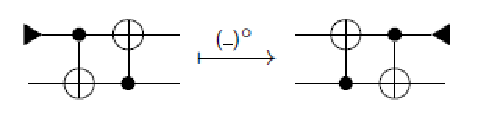
\includegraphics{CNOT.pdf}
\centering
\caption{Partial Inverse in the Category CNOT}
\end{figure}
CNOT is given by its generators and hence the proof involves many structural inductions


\section{Outline of the Proof}

\begin{theorem}
There is an equivalence of categories between CNOT and ParIso(CTor)$^{*}$
\end{theorem}
 \begin{enumerate}[(i)]
     \item Proof that CNOT is a discrete inverse category:\\
     For this one must  first construct a copy natural transformation $\Delta$ which is defined inductively. Then it has to be shown that $\Delta$ has the properties of an inverse product.
     \item Construction of a functor $\hat{H_{0}}: CNOT \to ParIso(CTor)^{*}$:\\
     In order to establish this we construct a functor $\hat{H_{0}}: CNOT \to ParIso(CTor_{2})^{*}$ indirectly by constructing a functor $H_{0}:CNOT \to Par(Set)$. We show that $H_{0}$ can be factored in two ways:
     \begin{itemize}
         \item Through the inclusion $\tau: ParIso(Set) \to Par(Set)$
         \item Through the underlying functor $Par(U): Par(CTor_{2})^{*} \to Par(Set)$.
     \end{itemize}
     These factorizations imply that $H_{0}$ factors through the pullbacks of $\tau$ and Par(U) which is $ParIso(CTor_{2})^{*}$. Thus we obtain the map $\hat{H_{0}}$. We must demonstrate that CNOT has an internal structure of to lift $h_{0}$ to the functor $\hat{H_{0}}: CNOT \to ParIso(CTor_{2})^{*}$. We define a $+: 3n \to 3n$ in CNOT which works as shown in the figure 5.
     \begin{figure}
         \centering
         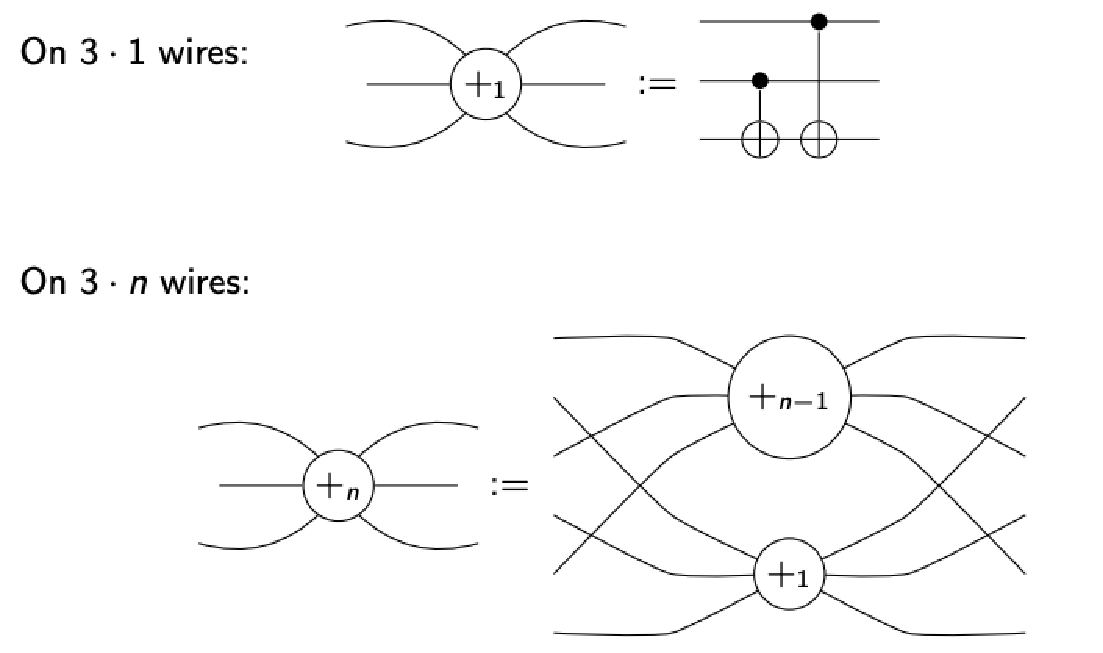
\includegraphics[scale=0.7]{torsor.pdf}
         \caption{Action of $+$}
         \label{fig:my_label}
     \end{figure}
     CNOT is a a freely generated symmetric monoidal category on the gates cnot, $\ket{1}$ and $\bra{1}$ it suffices to interpret these into the category $ParIso(CTor)^{*}$ and check all the identities hold.
     \item Proof that $H$ is a full and faithful functor:\\
     To show the faithfulness we reduce the problem to showing faithfulness on the restriction idempotents. To do this a causal form is introduced for restriction idempotents for CNOT.A circuit is in clausal form if and only if it is the composite of a finite
     number of clauses. A clause is a wire starting and ending with ancillary bits which is controlled
     from the identity (on n wires). Clauses correspond to torsor equations which can be manipulated using Gaussian elimination which implies that they are in bijective correspondance with the restriction idempotents. To obtain fullness we must show that any partial isomorphism between torsors can be simulated using circuits in CNOT. We first show that we can simulate the graph $\langle{1, f}\rangle$ of a total map $f$ between torsors. Next we note that any partial map between torsors is dominated by a total map, so we can simulate the graph of this total map. To introduce partiality we use the fact that the functor is full on restriction idempotents this allows us to simulate $\langle{\overline{f}, f}\rangle$ for any partial map $f$. However by a general result given in \cite{robin} we observe that simulating graphs of partial isomorphisms is sufficient to ensure we can simulate any partial isomorphism.
 \end{enumerate}
 

\begin{thebibliography}{10}
\bibitem{robin}Robin Cocket, Cole Comfort, Priyaa Srinivasan :The Category CNOT: EPTCS 266, 2018, pp. 258
\bibitem{brett}Brett Giles.
 An investigation of some theoretical aspects of reversible computing. PhD thesis, University of Calgary (2014)
\end{thebibliography}
\end{document}
